\section{Assignment 2}
\todo{Introduce assignment context and goals.}

\subsection{Stationary points}
For self-containment we repeat the MCM system of equations
\begin{align*}
    T^{\prime} & =r_1 T\left(1-\frac{T}{k_1}\right)-a_{12} T H-a_{13} T E, \\
    H^{\prime} & =r_2 H\left(1-\frac{H}{k_2}\right)-a_{21} T H, \\
    E^{\prime} & =\frac{r_3 T E}{T+k_3}-a_{31} T E-d_3 E ,
\end{align*}
and its dimensionless form
\begin{align*}
    & x_1^{\prime}=x_1\left(1-x_1\right)-p_1 x_1 x_2-p_2 x_1 x_3, \\
    & x_2^{\prime}=p_3 x_2\left(1-x_2\right)-p_4 x_1 x_2, \\
    & x_3^{\prime}=\frac{p_5 x_1 x_3}{x_1+p_6}-p_7 x_1 x_3-p_8 x_3 .
\end{align*}
The parameters $p_i$ are specified in Table \ref{tab:mcm_parameters}
\begin{table}[H]
    \centering
    \begin{tabular}{|c|c|c|c|}
        \hline
        Parameter   & Definition                & description           & Value \\
        \hline
        $p_1$       & $\frac{a_{12}k_2}{r_1}$     & T->H competition      & 0.5 \\
        $p_2$       & $\frac{a_{31}k_1}{r_1}$     & E->T killing          & 2.5 \\
        $p_3$       & $\frac{r_2}{r_1}      $     & H-T growth ratio      & 0.6 \\
        $p_4$       & $\frac{a_{21}k_1}{r_1}$     & T->H inactivation     & 1.5 \\
        $p_5$       & $\frac{r_3k_2}{r_1}   $     & T->E stimulation      & 4.5 \\
        $p_6$       & $\frac{k_3}{k_1}      $     & E-T capacity ratio    & 1.0 \\
        $p_7$       & $\frac{a_{31}k_3}{r_1}$     & T->E inactivation     & 0.2 \\
        $p_8$       & $\frac{d_3}{r_1}      $     & E natural death       & 0.5 \\
        \hline
    \end{tabular}
    \caption{Parameters of the dimensionless system}
    \label{tab:mcm_parameters}
\end{table}

\subsection{Continuation of stationary points}
Table \ref{tab:mcm_stationary_points} shows the stationary points of the system. 
\begin{table}[H]
	\begin{center}
		\begin{tabular}{|c|c|c|c|c|}
			\hline
			\textbf{index} & $\mathbf{x_1}$ & $\mathbf{x_2}$ & $\mathbf{x_3}$ & \textbf{stability} \\
			\hline
			1 & -2.00 & 6.00 & 0.00 & Unstable \\
			2 & 0.00 & 0.00 & 0.00 & Unstable \\
			3 & 0.00 & 1.00 & 0.00 & Unstable \\
			4 & 1.33$\times 10^{-1}$ & 0.00 & 3.47$\times 10^{-1}$ & Unstable \\
			5 & 1.33$\times 10^{-1}$ & 6.69$\times 10^{-1}$ & 2.13$\times 10^{-1}$ & Stable \\
			6 & 1.00 & 0.00 & 0.00 & Unstable \\
			7 & 1.89$\times 10^{1}$ & -4.62$\times 10^{1}$ & 2.09 & Unstable \\
			8 & 1.89$\times 10^{1}$ & 0.00 & -7.15 & Stable \\
			\hline
		\end{tabular}
	\end{center}
	\caption{Stationary points of the MCM model.}
	\label{tab:mcm_stationary_points}
\end{table}

We observe two stable stationary points (indices 5 and 8). We continue these
points in the parameter $ p_1 \in [0.5, 1] $ and plot the continuation in Figure \ref{fig:mcm_continuation}.
\begin{figure}[H]
    \centering
    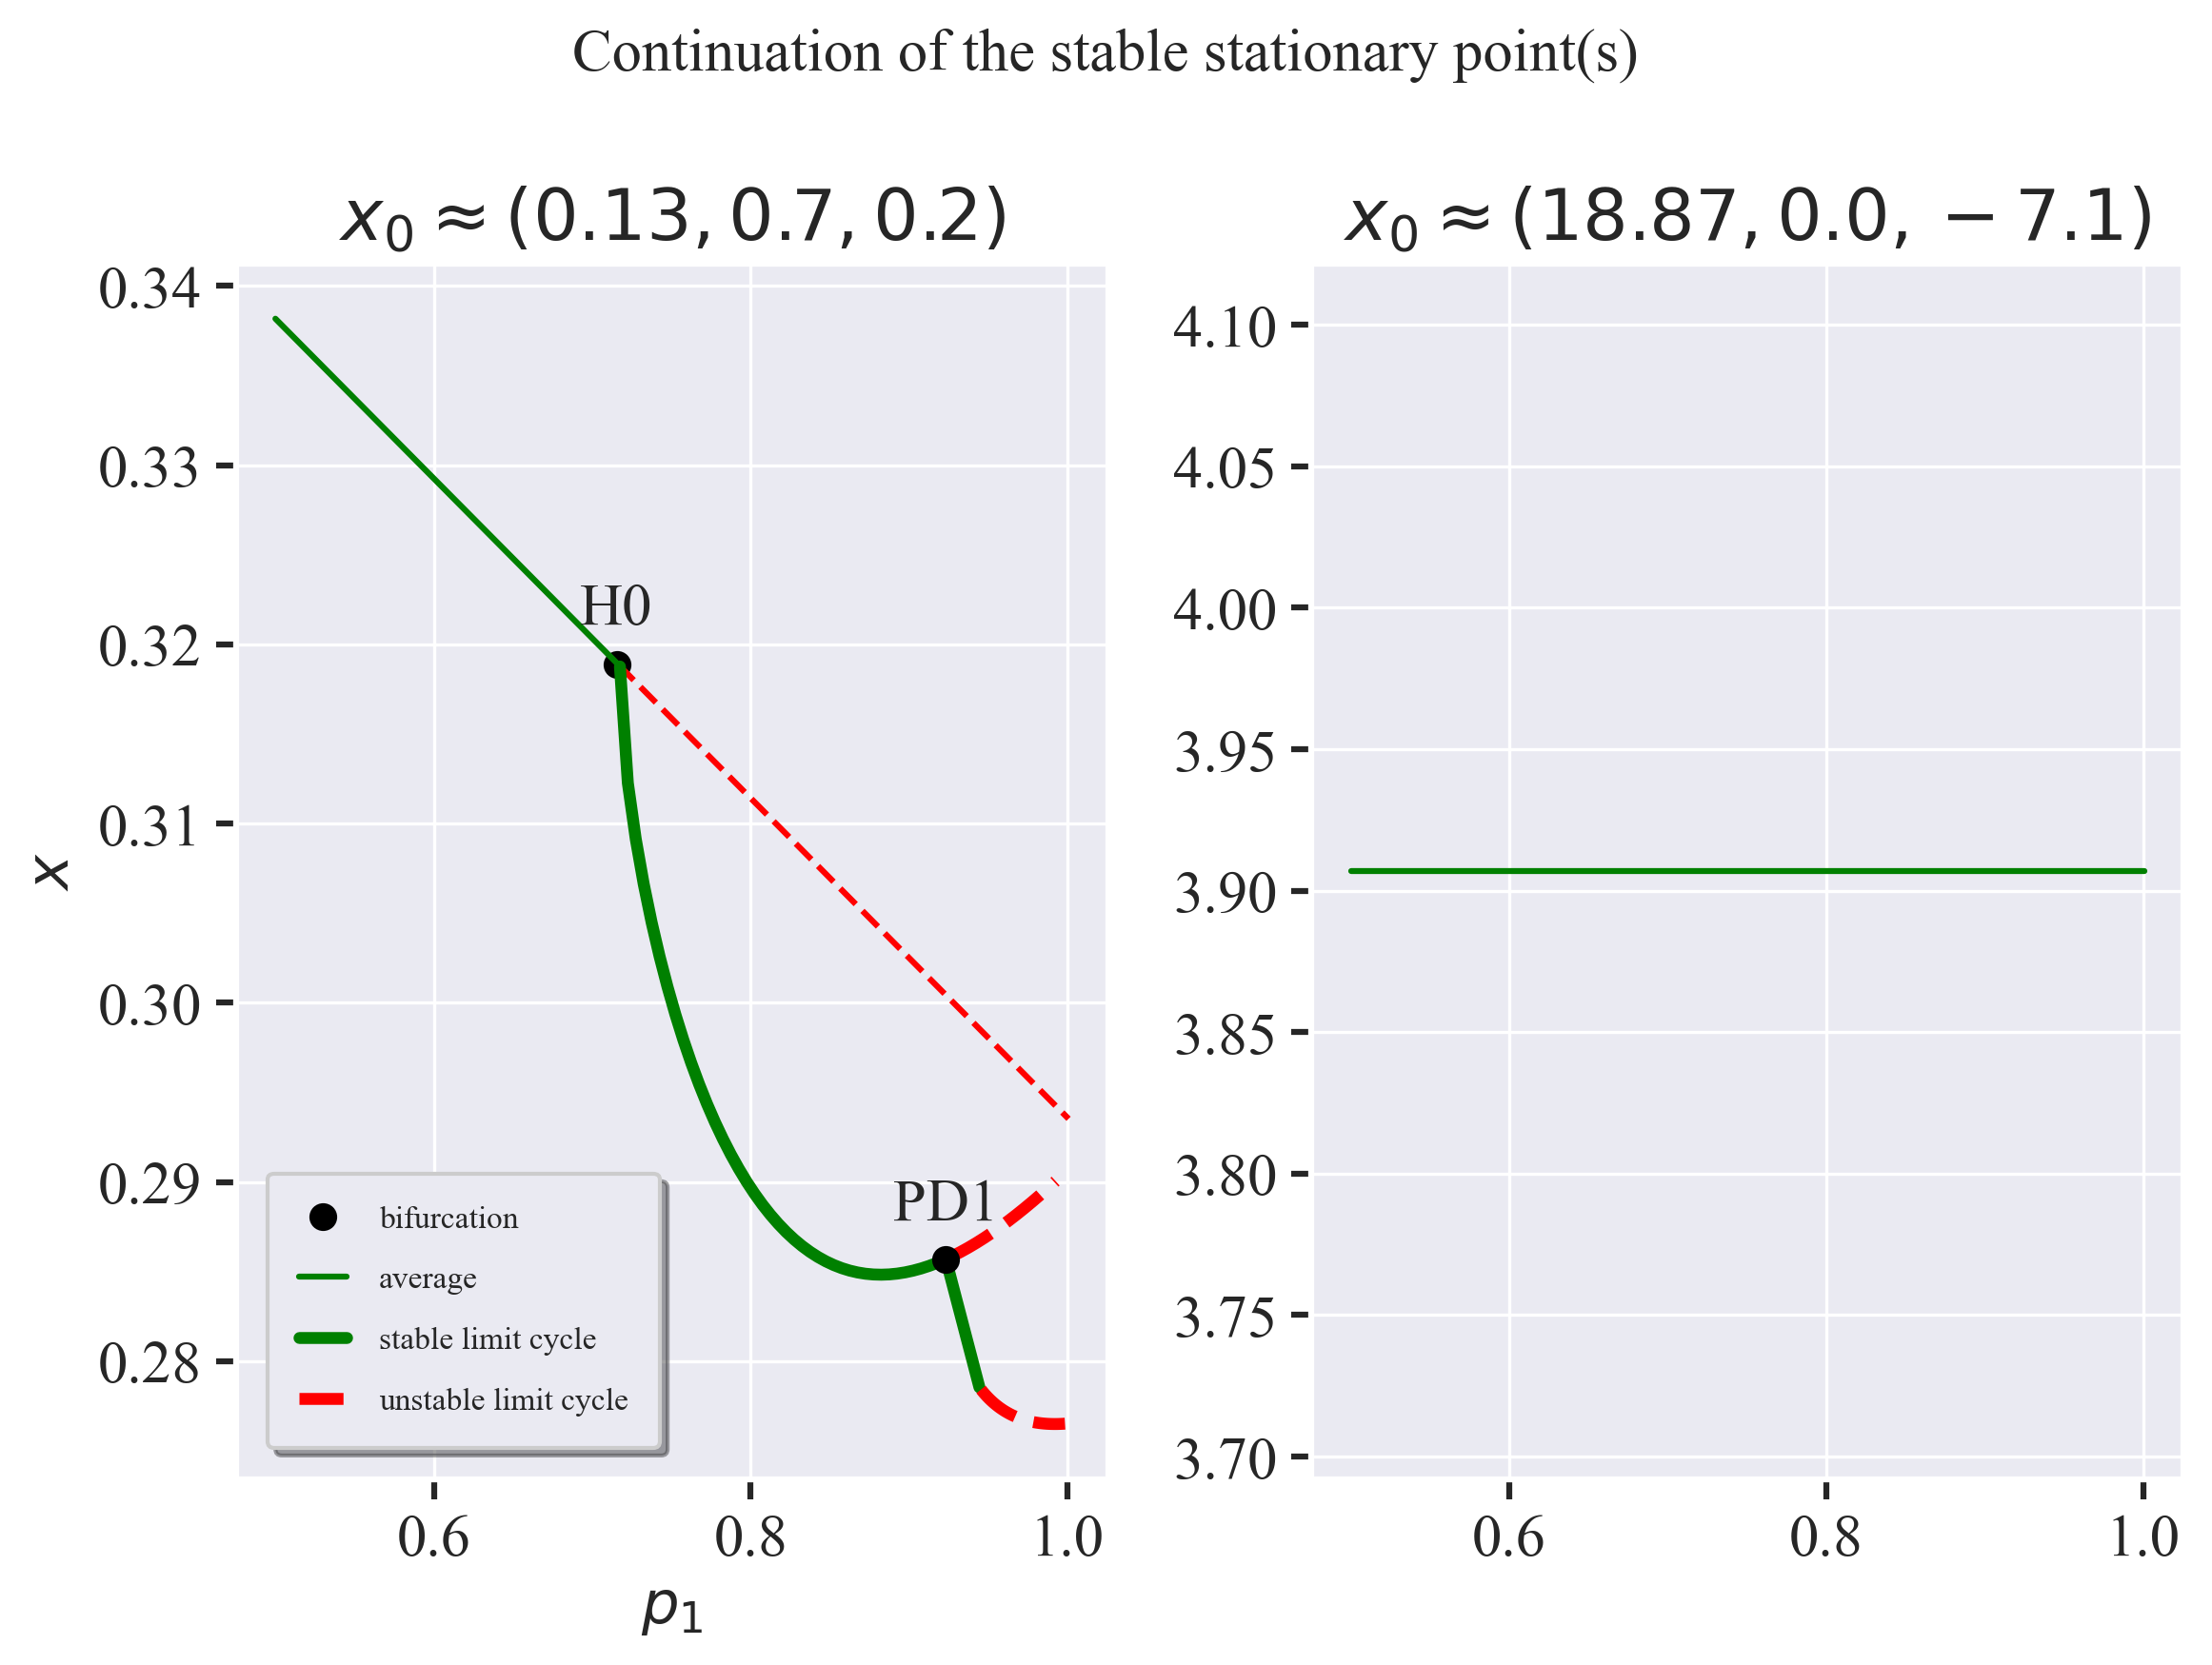
\includegraphics[width=0.8\textwidth]{figures/mcm_continuation.png}
    \caption{Continuation of the stable stationary points in the parameter $p_1$,
    point 5 (left) and point 8 (right). The former encounters a bifurcation at $p_1 \approx 0.71$}
    \label{fig:mcm_continuation}
\end{figure}

The bifurcation that occurs during the continuation of point 5 in Figure \ref{fig:mcm_continuation} is given by
\begin{align*}
    \text{Bifurcation type} & : subcritical(?) \text{Hopf} \\
    \text{Parameter} & : p_1 \\
    \text{Critical value} & : 0.71 \\
    \text{Eigenvalues} & : 0 \pm 0.36i, -0.53\\
    x_1, x_2, x_3 & : 0.13, 0.67, 0.16
\end{align*}
This bifurcation point was found by applying an indirect method based on the interpolation of test function values, adapted from 
Seydel's book (section 5.3.1). The particular test function used was the maximum of the real part of the eigenvalues of
the system Jacobian.

The bifurcation is a Hopf-bifurcation, as a complex pair of eigenvalues crosses the imaginary axis with non-zero velocity
That is to say, the eigenvalues of the system jacobian at the continuation step dircetly after the bifurcation are
\begin{align*}
    0.007 \pm 0.355i, -0.54
\end{align*},
which shows the eigenvalues pases through the imaginary axis with non-zero velocity.

Additionally, it is subcritical, as the emerging limit cycle is unstable (CHECK CHARACTERISATION). 

\todo{Calculate period of limit cycle.}

\subsection{Continuation of limit cycle}
\todo{describe continuation of limit cycle.}

\subsection{Period doubling bifurcations}
\todo{continue period doubling bifurcations.}
\todo{give formula to predict period doubling bifurcations.}

\subsection{Conclusion}
\todo{describe main results.}